\section{Experiments}
\label{sec:experiments}

\subsection{Experimental Setup}

\subsubsection{Dataset and Evaluation Metrics}
We evaluate our method on the Intentonomy dataset \cite{jia_intentonomy_2021}, a multi-label benchmark for visual intention recognition in social media scenarios. Following the standard split used in our experiments, the dataset contains 12,739 training images, 498 validation images, and 1,216 test images. Intentonomy additionally provides soft agreement annotations with values in $\{0, 0.33, 0.66, 1\}$ on the training set, which directly reflect the degree of annotator consensus and serve as the uncertainty signal $\omega$ in our framework.

We use Macro F1, Micro F1, Samples F1 as the evaluation metrics. To be consistent with recent Intentonomy works, we additionally report $\textit{Avg.}$, which is the average of three F1 scores. Unless otherwise stated, all reported numbers are percentages and all results are computed on the Intentonomy test split.

To better understand the effectiveness of our method, we further conduct experiments on subsets of the intent classes. We follow the work of Jia et al. \cite{jia_intentonomy_2021} and break down intent classes according to content difficulty and dependency. Difficulty classes are measured by how much a standard ResNet-50 model outperforms the random results. Content classes are divided into object-dependent ({\itshape Object}-classes), context-dependent ({\itshape Context}-classes), and {\itshape Others}, which depend on both foreground and background information. We emphasize the \textit{Hard} score throughout the analysis because it specifically measures performance on ambiguity-prone intent categories, where semantic overlap and subjective disagreement are most severe. Improvements on the hard subset therefore provide stronger evidence that a method is resolving the core difficulty of intention understanding rather than merely exploiting easy classes.

\begin{table}[htbp]
\centering
\small
\caption{Main comparison on Intentonomy test split. Avg.\ is the mean of Macro/Micro/Samples F1. FDIL rows report mean$\pm$std over three seeds. $^{\dagger}$Quoted from IntentMLM~\cite{wang_unlocking_2026}.}
\label{tab:main_results}
\begingroup
\setlength{\tabcolsep}{4pt}
\begin{tabular}{llcccc}
\hline
Method & Publication & Macro F1 & Micro F1 & Samples F1 & Avg. \\
\hline
Random & - & 6.94 & 7.18 & 7.10 & 7.07 \\
Visual \cite{he_deep_2016} & CVPR 2016 & 22.77 & 30.23 & 28.45 & 27.15 \\
\hline
\multicolumn{6}{l}{\textbf{Multi-label classification methods}} \\
HiMulConE \cite{zhang_use_2022} & CVPR 2022 & 28.43 & 41.50 & 42.15 & 37.36 \\
MultiGuard \cite{jia_multiguard_2022} & NeurIPS 2022 & 26.87 & 38.67 & 40.06 & 35.20 \\
SST \cite{chen_structured_2022} & AAAI 2022 & 27.33 & 42.21 & 42.62 & 37.39 \\
Query2Label \cite{liu_query2label_2021} & - & 32.12 & 44.64 & 45.15 & 40.64 \\
DualCoOp \cite{sun_dualcoop_2022} & NeurIPS 2022 & 31.06 & 44.42 & 40.40 & 38.63 \\
\hline
\multicolumn{6}{l}{\textbf{Label noise methods}} \\
Cleannet \cite{lee_cleannet_2018} & CVPR 2018 & 25.89 & 42.15 & 40.97 & 36.34 \\
LS \cite{lukasik_does_2020} & ICML 2020 & 24.32 & 42.77 & 43.27 & 36.79 \\
Dividemix \cite{li_dividemix_2019} & ICLR 2020 & 30.11 & 40.23 & 41.56 & 37.30 \\
\hline
\multicolumn{6}{l}{\textbf{Intent perception methods}} \\
Jia \cite{jia_intentonomy_2021} & CVPR 2021 & 23.98 & 31.28 & 31.39 & 28.88 \\
CPAD \cite{ye_cross-modality_2023} & TIP 2023 & 27.39 & 40.98 & 41.12 & 36.50 \\
HLEG \cite{shi_learnable_2023} & TAC 2023 & 32.77 & 44.69 & 45.54 & 41.00 \\
HLEG (CLIP ViT-L/14) \cite{shi_learnable_2023} & TAC 2023 & 48.17 & 57.29 & 56.81 & 54.09 \\
PIP-Net \cite{wang_prototype-based_2023} & TMM 2023 & 32.57 & 45.94 & 47.05 & 41.85 \\
LabCR \cite{shi_label-aware_2024} & TIP 2024 & 34.63 & 48.51 & 48.05 & 43.73 \\
LabCR (CLIP ViT-L/14) \cite{shi_label-aware_2024} & TIP 2024 & 48.04 & 57.13 & 56.65 & 53.94 \\
IntCLIP \cite{leonardis_synergy_2025} & ECCV 2024 & 40.15 & 53.54 & 51.01 & 48.23 \\
IntCLIP (CLIP ViT-L/14) \cite{leonardis_synergy_2025} & ECCV 2024 & 47.28 & 56.18 & 54.86 & 52.77 \\
% \hline
% \multicolumn{6}{l}{\textbf{Multimodal large model methods}} \\
% Qwen2-VL-7B & - & 21.85 & 27.06 & 33.48 & 27.46 \\
% Ovis1.6-Gemma2-9B & - & 36.14 & 34.52 & 33.93 & 34.86 \\
% GPT-4o & - & 39.48 & 40.57 & 41.45 & 40.50 \\
IntentMLM \cite{wang_unlocking_2026} & PR 2026 & 43.05 & 54.77 & 56.75 & 51.52 \\
\hline
\multicolumn{6}{l}{\textbf{Zero-shot VLM}} \\
Qwen3-VL-8B-Instruct \cite{qwen_qwen3-vl_2025} & - & 38.51 & 40.75 & 39.63 & 39.63 \\
InternVL3-8B \cite{zhu_internvl3_2025} & - & 37.54 & 41.85 & 40.50 & 39.97 \\
GPT-4o \cite{hurst_gpt-4o_2024}$^{\dagger}$ & - & 39.48 & 40.57 & 41.45 & 40.50 \\
\hline
CLIP ViT-L/14 \cite{radford_learning_2021} & ICML 2021 & $47.40$ & $56.42$ & $56.41$ & $53.41$ \\
FDIL (UTD only) & Ours & $50.20_{\pm0.44}$ & $58.03_{\pm0.11}$ & $58.79_{\pm0.78}$ & $55.68_{\pm0.44}$ \\
FDIL & Ours & $\mathbf{52.13}_{\pm0.81}$ & $\mathbf{60.06}_{\pm0.24}$ & $\mathbf{60.28}_{\pm0.42}$ & $\mathbf{57.49}_{\pm0.49}$ \\
\hline
\end{tabular}
\endgroup
\end{table}

\subsubsection{Implementation Details}

Our default visual backbone is frozen CLIP ViT-L/14 \cite{radford_learning_2021}. The visual student is implemented as a lightweight residual MLP trained on top of a fixed SLR-C prior. In SLR-C, priors are constructed from three sources, namely lexical intent phrases, canonical intent descriptions, and Gemini 3.1 Pro-generated scenario descriptions \cite{team_gemini_2025} with frozen CLIP text encoder \cite{radford_learning_2021}; their normalized logits are averaged before local reranking within Top-10 visual candidates. For UTD, rationale text is generated offline by Qwen2.5-VL-7B-Instruct \cite{bai_qwen25-vl_2025} and then encoded by a frozen bge-large-en-v1.5 text encoder \cite{xiao_c-pack_2024}. The exact scenario- and rationale-generation prompt templates are released together with our artifacts. The teacher consumes only the resulting text embeddings and is optimized with Asymmetric Loss (ASL) \cite{ridnik_asymmetric_2021} using $\gamma_{-}=2$, $\gamma_{+}=0$, and clipping value 0.05. The student is optimized with AdamW \cite{loshchilov_decoupled_2018}, learning rate $5\times10^{-4}$, weight decay $10^{-4}$, batch size 256, and dropout 0.1. The teacher's hidden dimension is 1,024, and the student's hidden dimension is 768. The distillation temperature is set to 2.0. Best-epoch selection and early stopping use validation class-wise Macro F1 only. All decision thresholds are fitted exclusively on the validation split and then fixed before test evaluation; test outputs are used solely for final reporting and never enter any model- or threshold-selection branch. Notably, UTD introduces \emph{zero extra inference cost}, since the text teacher is only used during training and is discarded at test time.

\subsection{Comparative Experiments}

\subsubsection{Comparison with state-of-the-art methods}

Table~\ref{tab:main_results} summarizes the main comparison on the test split. The strong CLIP baseline already surpasses the previously reported best result by a clear margin; however, because the previous methods are quoted under their original, generally weaker backbones, this margin mainly reflects backbone strength rather than algorithmic superiority, and we therefore do not interpret it as evidence for FDIL. For a fair comparison, we additionally reproduce the core mechanism of representative recent methods over the same frozen CLIP ViT-L/14 features, split, and validation-only class-wise thresholding, shown as the ``(CLIP ViT-L/14)'' rows. Under this matched protocol FDIL still leads all of them by $+3.4$ to $+4.7$ average F1. Building on the same features, UTD alone improves the average F1 over the baseline at zero extra inference cost, and the full FDIL framework further improves all four metrics. This pattern is consistent with our motivation that fixed semantic priors supply structured candidate semantics while uncertainty-aware supervision and image-aware refinement sharpen the final prediction.

\subsubsection{Zero-shot Multimodal Large Model Comparison}

To address the concern that recent multimodal large language models may already solve visual intent recognition through prompting alone, we evaluate two recent open-weight MLLMs zero-shot on the same Intentonomy label set, prompting each to return a probability over the candidate categories; the group additionally lists, for reference, the GPT-4o zero-shot result reported by IntentMLM~\cite{wang_unlocking_2026}. As shown in the \textit{Zero-shot VLM} group of Table~\ref{tab:main_results}, direct zero-shot prediction is competitive but remains below the trained CLIP and FDIL models. Stronger general-purpose MLLMs therefore provide useful intent priors, but prompt-only recognition does not remove the need for dataset-specific calibration, uncertainty-aware supervision, and image-conditioned refinement.

\subsubsection{Performance on Difficulty- and Content-Dependent Subsets}

To better understand the effectiveness of our method, we further evaluate performance on intent subsets grouped by difficulty (Table~\ref{tab:difficulty_results}) and by content dependency (Table~\ref{tab:content_results}). The difficulty-wise results provide two additional insights. First, the CLIP baseline already matches or exceeds prior methods across the three difficulty groups; on the easy subset FDIL is the stronger of our two models and trails only HLEG by $0.30$, a negligible gap on visually unambiguous categories where modelling semantic overlap offers little headroom. Second, FDIL yields its largest and most consistent gains on the medium and hard subsets, precisely where semantic ambiguity and supervisory uncertainty are most pronounced and which the framework is designed to target.
% Validation-split results are omitted to respect the page limit (reported in the response letter).

\begin{table}[htbp]
\centering
\caption{Difficulty-based intent subsets (Easy/Medium/Hard); Avg.\ is the subset mean. FDIL is the mean over three seeds.}
\label{tab:difficulty_results}
\begin{tabular}{lcccc}
\hline
Method & Easy & Medium & Hard & Avg. \\
\hline
Random & 19.86 & 7.11 & 2.81 & 9.93 \\
Visual \cite{he_deep_2016} & 54.64 & 24.92 & 10.71 & 30.09 \\
Jia (w/o hashtag) \cite{jia_intentonomy_2021} & 57.10 & 25.68 & 12.72 & 31.83 \\
Jia (hashtag) \cite{jia_intentonomy_2021} & 58.86 & 26.30 & 13.11 & 32.76 \\
Query2Label \cite{liu_query2label_2021} & 81.59 & 38.06 & 14.55 & 44.73 \\
CPAD \cite{ye_cross-modality_2023} & 69.47 & 31.50 & 8.54 & 36.50 \\
HLEG \cite{shi_learnable_2023} & 81.49 & 38.99 & 20.22 & 46.90 \\
PIP-Net \cite{wang_prototype-based_2023} & 70.73 & 33.63 & 14.33 & 39.56 \\
IntentMLM \cite{wang_unlocking_2026} & 76.26 & 46.87 & 27.39 & 50.17 \\
\hline
CLIP ViT-L/14 \cite{radford_learning_2021} & 80.99 & 53.32 & 28.45 & 54.25 \\
FDIL & \textbf{81.19} & \textbf{57.73} & \textbf{35.02} & \textbf{57.98} \\
\hline
\end{tabular}
\end{table}

\begin{table}[htbp]
\centering
\caption{Content-dependent intent subsets (Object/Context/Others); Avg.\ is the subset mean. FDIL is the mean over three seeds.}
\label{tab:content_results}
\begin{tabular}{lcccc}
\hline
Method & Object & Context & Others & Avg. \\
\hline
Random & 7.75 & 12.53 & 6.05 & 8.78 \\
Visual \cite{he_deep_2016} & 25.58 & 30.16 & 21.34 & 25.69 \\
Jia (w/o hashtag) \cite{jia_intentonomy_2021} & 28.15 & 28.62 & 22.60 & 26.46 \\
Jia (hashtag) \cite{jia_intentonomy_2021} & 29.66 & 32.48 & 22.61 & 28.25 \\
CPAD \cite{ye_cross-modality_2023} & 28.81 & 47.30 & 24.74 & 33.62 \\
PIP-Net \cite{wang_prototype-based_2023} & 39.20 & 39.53 & 27.59 & 35.44 \\
IntentMLM \cite{wang_unlocking_2026} & 50.13 & 49.69 & 39.75 & 46.52 \\
\hline
CLIP ViT-L/14 \cite{radford_learning_2021} & 61.80 & \textbf{61.69} & 40.59 & 54.69 \\
FDIL & \textbf{63.04} & 61.32 & \textbf{47.15} & \textbf{57.17} \\
\hline
\end{tabular}
\end{table}

Turning to content dependency, Table~\ref{tab:content_results} reports results on content-dependent subsets.
It again shows that the strong CLIP baseline is already highly effective on object- and context-dependent intents. The major gain of FDIL appears in the \textit{Others} subset, where intent recognition requires more holistic reasoning over multiple weak cues rather than direct reliance on a single object or scene pattern.
% Validation-split results are omitted to respect the page limit (reported in the response letter).

\subsubsection{Interpretability Analysis}

To make the source of the improvement interpretable rather than aggregate, we examine where in the label space FDIL helps. Figure~\ref{fig:tsne} shows a t-SNE projection of the decision-score space on four semantically adjacent intents: FDIL produces more compact, better-separated same-intent clusters than the CLIP baseline (silhouette $0.21\!\to\!0.29$), indicating that the semantic prior and the rationale teacher together pull confusable neighboring intents apart rather than merely rescaling scores. We further compute the per-class F1 change of FDIL relative to the CLIP baseline under the matched class-wise protocol. The largest per-class gains are concentrated on hard and abstract classes, including \textit{WorkILike} ($+28.5$), \textit{PassionAboutSomething} ($+17.3$), and \textit{SocialLifeFriendship} ($+17.2$), while only two classes regress.

\begin{figure}[htbp]
\centering
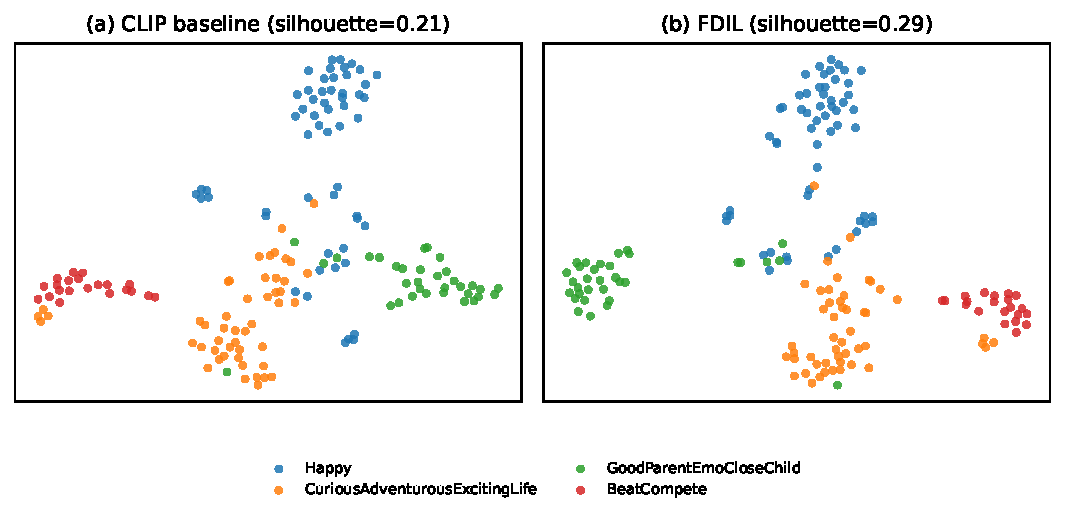
\includegraphics[width=0.9\linewidth]{5_tsne.pdf}
\caption{t-SNE of the decision-score space on four semantically adjacent intents. FDIL yields tighter, better-separated same-intent clusters than the CLIP baseline.}
\label{fig:tsne}
\end{figure}

%% --- BEGIN condensed-out for 35-page limit: per-class attribution table moved to response letter ---
%% (Full per-class F1 attribution table relocated to the response letter; the
%%  main-text one-sentence summary above retains the key per-class gains.)
\iffalse
We further compute the per-class F1 change of FDIL relative to the CLIP baseline under the matched class-wise protocol (Table~\ref{tab:per_class_attr}). The gains are strongly concentrated on abstract, disagreement-prone intents -- \textit{WorkILike}, \textit{PassionAboutSomething}, and \textit{SocialLifeFriendship} (all hard-subset classes), together with \textit{ManageableMakePlan} and \textit{BeatCompete}, each improve by more than $13$ F1 points -- which are precisely the categories where semantic overlap and supervisory ambiguity are most severe. Crucially, only $2$ of the $28$ classes regress at all: \textit{FineDesignLearnArt-Arch} drops by a negligible $0.96$, and the only non-trivial regression is \textit{CreativeUnique} ($-5.3$), a broad ``creative/unique'' category that overlaps heavily with several neighboring design- and art-related intents and that the residual student occasionally resolves toward a competing neighbor. No easy or visually clear category is otherwise harmed, so the per-class calibration does not trade broad accuracy for hard-case robustness.

\begin{table}[htbp]
\centering
\small
\caption{Per-class F1 attribution of FDIL versus the CLIP baseline (matched class-wise protocol, representative seed). Top: five largest improvements; bottom: the only two regressions among all $28$ classes.}
\label{tab:per_class_attr}
\setlength{\tabcolsep}{5pt}
\begin{tabular}{lcccc}
\hline
Intent class & Subset & Baseline & FDIL & $\Delta$ \\
\hline
WorkILike & Hard & 14.6 & 43.0 & $+28.5$ \\
PassionAboutSomething & Hard & 11.3 & 28.6 & $+17.3$ \\
SocialLifeFriendship & Hard & 33.9 & 51.2 & $+17.2$ \\
ManageableMakePlan & Medium & 17.5 & 32.0 & $+14.5$ \\
BeatCompete & Medium & 54.6 & 68.1 & $+13.5$ \\
\hline
FineDesignLearnArt-Arch & Easy & 84.0 & 83.1 & $-1.0$ \\
CreativeUnique & Medium & 41.9 & 36.6 & $-5.3$ \\
\hline
\end{tabular}
\end{table}
\fi
%% --- END condensed-out for 35-page limit ---

\subsection{Ablation Studies}

\subsubsection{Effectiveness of SLR-C and Residual Refinement}

We first study how SLR-C interacts with residual learning and distillation. Table~\ref{tab:slrc_ablation} shows that prior alone is insufficient, while adding a trainable student and distillation is essential for recovering robust intent predictions.
\begin{table}[htbp]
\centering
\caption{Component ablation of FDIL (\textit{w/o UTD}: no text distillation; \textit{w/o Gated}: no agreement-aware gating). Full FDIL is the mean over three seeds; ablations use a single seed.}
\label{tab:slrc_ablation}
\begin{tabular}{lccccc}
\hline
Method & Macro & Micro & Samples & Avg. & Hard \\
\hline
w/o UTD & 47.90 & 55.98 & 55.18 & 53.02 & 29.71 \\
w/o Gated & 49.69 & 57.90 & 58.98 & 55.52 & 31.69 \\
FDIL (full) & \textbf{52.13} & \textbf{60.06} & \textbf{60.28} & \textbf{57.49} & \textbf{35.02} \\
\hline
\end{tabular}
\end{table}

Two observations are noteworthy. First, naively injecting a heterogeneous prior is not enough; without a trainable student, the mixed prior can distort the score geometry and lead to poor predictions. Second, once distillation is introduced, residual refinement becomes consistently beneficial, showing that heterogeneous prior fusion and uncertainty-aware supervision must be optimized jointly rather than independently.

\subsubsection{Unified versus Functionally Decoupled Ambiguity Handling}

We next examine whether the functional decomposition is necessary, or whether a single unified mechanism can absorb both forms of ambiguity. Table~\ref{tab:unified_decoupled} contrasts the decoupled FDIL model with three unified controls under identical frozen CLIP ViT-L/14 features, data split, and validation-only class-wise thresholding. The most direct control, \textit{Unified joint-target KD}, averages the SLR-C and rationale-teacher probabilities into a single distillation target and trains one image-feature student, without residual decomposition or agreement-aware gating.

\begin{table}[htbp]
\centering
\small
\caption{Unified versus functionally decoupled ambiguity handling. Results are means over three seeds.}
\label{tab:unified_decoupled}
\setlength{\tabcolsep}{4pt}
\begin{tabular}{lccccc}
\hline
Method & Macro & Micro & Samples & Avg. & Hard \\
\hline
Unified UTD only & 50.20 & 58.03 & 58.79 & 55.68 & 30.27 \\
Unified SLR-C only & 51.29 & \textbf{60.10} & 59.22 & 56.87 & 34.01 \\
Unified joint-target KD & 50.69 & 58.35 & 57.96 & 55.66 & 32.41 \\
FDIL (decoupled) & \textbf{52.13} & 60.06 & \textbf{60.28} & \textbf{57.49} & \textbf{35.02} \\
\hline
\end{tabular}
\end{table}

The results show that neither signal is degenerate in isolation: the semantic prior alone and the rationale teacher alone are each competitive. Crucially, the manner of combination is decisive. Collapsing the two signals into a single mixed target (\textit{Unified joint-target KD}) yields no benefit, whereas the decoupled FDIL model is best overall. We therefore interpret decoupling as conferring a small but consistent accuracy gain over a single mixed target, together with its primary advantage of modularity: each function is separately justified and measurable, yielding an independent mAP increment, and the UTD branch can be deployed alone at zero additional inference cost.

\subsubsection{Heterogeneous Priors in SLR-C}

We next compare different textual priors used by SLR-C. We consider three semantic sources: \textit{Lexical}, which uses short class-name phrases; \textit{Canonical}, which uses the official intent descriptions provided by Intentonomy; and \textit{Scenario}, which uses Gemini-generated visual scenarios. For the ensemble setting, we average the normalized logits from the selected sources before local reranking. Table~\ref{tab:prior_ablation} therefore isolates the effect of prior sources under the SLR-C reranking stage only.
\begin{table}[htbp]
\centering
\caption{Ablation of textual priors in SLR-C (reranking-only, $K{=}10$). Results use a single seed.}
\label{tab:prior_ablation}
\begin{tabular}{cccccccc}
\hline
Lexical & Canonical & Scenario & Macro & Micro & Samples & Avg. & Hard \\
\hline
$\checkmark$ &  &  & 49.76 & 59.12 & \textbf{58.60} & 55.83 & 31.22 \\
 & $\checkmark$ &  & 49.80 & 59.50 & 58.05 & 55.78 & 29.88 \\
 &  & $\checkmark$ & 49.35 & 58.88 & 57.87 & 55.37 & 32.48 \\
$\checkmark$ & $\checkmark$ &  & \textbf{51.18} & 59.39 & 58.11 & 56.23 & 32.92 \\
$\checkmark$ &  & $\checkmark$ & 50.12 & 59.30 & 58.36 & 55.93 & 32.75 \\
 & $\checkmark$ & $\checkmark$ & 50.93 & 59.51 & 58.18 & 56.21 & \textbf{34.81} \\
$\checkmark$ & $\checkmark$ & $\checkmark$ & 50.90 & \textbf{59.81} & 58.47 & \textbf{56.40} & 32.80 \\
\hline
\end{tabular}
\end{table}

The results show that ensemble outperforms its single-source components on the aggregate metrics, confirming that the three sources carry complementary information. Lexical phrases are compact, canonical descriptions are semantically explicit, and scenario descriptions ground latent intention into typical visual situations. Second, no single source dominates at the reranking-only stage, the choice of prior is a trade-off rather than a strict ordering. Third, the three-source ensemble achieves the best aggregate performance and the broadest semantic coverage, and once combined with residual refinement and the UTD teacher it also yields the strongest hard-subset result. We therefore adopt it in FDIL for its balanced coverage and strong behaviour under the full pipeline.

\subsubsection{Sensitivity to Candidate Size $K$}

We next study the effect of candidate size $K$ while fixing the thresholding strategy to the final class-wise setting. Table~\ref{tab:k_sensitivity_test} reports the test-split results obtained by retraining FDIL under $K \in \{5,10,28\}$ and then searching thresholds on the validation split. The comparison shows that the best overall result is achieved at $K=10$, which we adopt as the default candidate size; $K=5$ is slightly weaker and $K=28$ is comparable but offers no further benefit. This suggests that, under the final lexical-canonical-scenario prior, a moderate local candidate set best balances semantic coverage against the distractor noise introduced by an overly broad reranking range.

\begin{table}[htbp]
\centering
\caption{Sensitivity to candidate size $K$ (class-wise thresholding). Results are means over three seeds.}
\label{tab:k_sensitivity_test}
\begin{tabular}{lccccc}
\hline
Top-$K$ & Macro & Micro & Samples & Avg. & Hard \\
\hline
5 & 51.19 & 59.03 & 59.42 & 56.54 & 31.60 \\
10 & \textbf{52.13} & \textbf{60.06} & \textbf{60.28} & \textbf{57.49} & \textbf{35.02} \\
28 & 51.64 & 59.59 & 59.71 & 56.98 & 34.02 \\
\hline
\end{tabular}
\end{table}

\begin{table}[htbp]
\centering
\small
\caption{Calibration decomposition under matched global/class-wise thresholding. FDIL is mean$\pm$std over three seeds; CLIP uses a single seed.}
\label{tab:thresholding_test}
\setlength{\tabcolsep}{3pt}
\begin{tabular}{llcccccc}
\hline
Method & Threshold & Macro & Micro & Samples & Avg. & mAP & Hard \\
\hline
CLIP ViT-L/14 \cite{radford_learning_2021} & Global & $46.22$ & $55.05$ & $54.51$ & $51.92$ & $50.67$ & $26.84$ \\
CLIP ViT-L/14 \cite{radford_learning_2021} & Class-wise & $47.40$ & $56.42$ & $56.41$ & $53.41$ & $50.67$ & $28.45$ \\
\hline
FDIL & Global & $47.70_{\pm1.55}$ & $57.56_{\pm0.41}$ & $57.43_{\pm0.69}$ & $54.23_{\pm0.72}$ & $\mathbf{55.10}_{\pm0.26}$ & $30.00_{\pm3.46}$ \\
FDIL & Class-wise & $\mathbf{52.13}_{\pm0.81}$ & $\mathbf{60.06}_{\pm0.24}$ & $\mathbf{60.28}_{\pm0.42}$ & $\mathbf{57.49}_{\pm0.49}$ & $\mathbf{55.10}_{\pm0.26}$ & $\mathbf{35.02}_{\pm1.77}$ \\
\hline
\end{tabular}
\end{table}

\subsubsection{Calibration and Threshold-free Evaluation}

To separate FDIL's mechanisms from class-wise calibration, we evaluate both the CLIP baseline and FDIL under matched global and class-wise thresholding (Table~\ref{tab:thresholding_test}). FDIL improves over the baseline under both protocols on average and hard-subset F1, and class-wise thresholding helps both models, so calibration is a shared post-processing gain rather than the source of FDIL's advantage. The threshold-free mAP, invariant to the decision rule by construction, confirms the same conclusion with a $+4.4$ gain.

\begin{table}[htbp]
\centering
\small
\caption{Threshold-free, rank-based metrics. mAP is the macro average precision. FDIL/UTD mAP values are means over three seeds; all AUCs and CLIP mAP use a single representative seed.}
\label{tab:threshold_free}
\setlength{\tabcolsep}{4pt}
\begin{tabular}{lcccc}
\hline
Method & mAP & Macro ROC-AUC & Micro ROC-AUC & Micro PR-AUC \\
\hline
CLIP ViT-L/14 \cite{radford_learning_2021} & 50.67 & 87.04 & 84.90 & 54.89 \\
UTD only & 53.07 & \textbf{90.09} & \textbf{88.55} & 59.59 \\
SLR-C only & 53.79 & 88.24 & 86.73 & 58.60 \\
FDIL & \textbf{55.10} & 89.36 & 88.31 & \textbf{60.64} \\
\hline
\end{tabular}
\end{table}

\begin{figure}[htbp]
\centering

\includegraphics[width=0.9\linewidth]{4_roc_pr.pdf}
\caption{Micro-averaged ROC (a) and precision-recall (b) curves, comparing FDIL against the CLIP baseline and three representative methods (HLEG, LabCR, IntCLIP) reproduced under the matched CLIP ViT-L/14 features, split, and protocol.}
\label{fig:roc_pr}
\end{figure}

Table~\ref{tab:threshold_free} and Figure~\ref{fig:roc_pr} report fully threshold-free, rank-based metrics (mAP, ROC-AUC, PR-AUC) for FDIL, its ablations, and representative methods reproduced under the matched CLIP ViT-L/14 protocol. FDIL improves over the baseline on every metric with a $95\%$ paired-bootstrap interval excluding zero ($p<0.001$), and FDIL outperforms the reproduced methods when the backbone is equalized.

\subsubsection{The Effectiveness of Rationale}

We then compare generic image captioning with rationale-style supervision under UTD only setting. We further ablate the internal structure of the rationale used by the text teacher. Specifically, we compare Caption, which only describes visible content in short natural language; Step 1 only, which contains observable visual evidence; Step 1 with Step 2, which additionally introduces contextual interpretation; and Full rationale, which further adds counterfactual disambiguation cues. Table~\ref{tab:rationale_ablation} reports the results under gated distillation without SLR-C.
\begin{table}[htbp]
\centering
\caption{Ablation of rationale construction for UTD (Step 1/2/3: visual evidence, contextual bridging, counterfactual disambiguation). Results use a single seed.}
\label{tab:rationale_ablation}
\begin{tabular}{lccccc}
\hline
Method & Macro & Micro & Samples & Avg. & Hard \\
\hline
Caption & 49.64 & \textbf{58.64} & 58.29 & 55.52 & 29.14 \\
Rationale (Step 1) & 49.81 & 56.39 & 57.65 & 54.62 & 29.28 \\
Rationale (Step 1 \& 2) & 49.69 & 54.45 & 55.97 & 53.37 & 28.82 \\
Rationale (Step 1 \& 2 \& 3) & \textbf{50.31} & 57.97 & \textbf{59.07} & \textbf{55.78} & \textbf{30.24} \\
\hline
\end{tabular}
\end{table}

The trend is revealing. Caption supervision is already a reasonably strong privileged signal, but it remains slightly weaker than the full rationale in Macro, Samples, Avg., and Hard. Step 1 already provides useful visual facts, but adding Step 2 alone slightly degrades the overall classification metrics, suggesting that contextual interpretation without explicit disambiguation may introduce semantic drift. Once the counterfactual Step 3 is added, however, the rationale becomes significantly more effective. This supports our central claim that subjective intention recognition requires not only richer context, but also explicit boundary contraction among confusing alternatives.

\subsubsection{UTD Ablations: Gating and Teacher Modality}

We isolate the effect of UTD without using the SLR-C prior, jointly studying agreement-aware gating and the teacher's input modality. Table~\ref{tab:utd_ablation} (top block) compares plain supervised learning, distillation without gating, and agreement-aware gated distillation; the bottom block contrasts teacher-only oracle performance with the corresponding gated-distillation student under text-only versus image+text teacher inputs.
\begin{table}[htbp]
\centering
\small
\caption{UTD teacher ablations without SLR-C. Top: agreement-aware gating. Bottom: teacher input modality (oracle and gated student). Results use a single seed; bold marks the best entry within each comparison.}
\label{tab:utd_ablation}
\setlength{\tabcolsep}{4pt}
\begin{tabular}{llccccc}
\hline
Method & Modality & Macro & Micro & Samples & Avg. & Hard \\
\hline
\multicolumn{7}{l}{\textit{Effect of agreement-aware gating}} \\
Baseline & -- & 47.40 & 56.42 & 56.41 & 53.41 & 28.45 \\
UTD (w/o gated) & Text & 49.59 & \textbf{58.26} & 58.88 & 55.58 & \textbf{30.44} \\
UTD (with gated) & Text & \textbf{50.31} & 57.97 & \textbf{59.07} & \textbf{55.78} & 30.24 \\
\hline
\multicolumn{7}{l}{\textit{Effect of teacher input modality}} \\
Oracle teacher & Text & 45.80 & 51.42 & 52.61 & 49.94 & \textbf{30.21} \\
Oracle teacher & Image+Text & 45.87 & 53.44 & 54.04 & 51.12 & 28.08 \\
Gated student & Text & \textbf{50.31} & \textbf{57.97} & \textbf{59.07} & \textbf{55.78} & \textbf{30.24} \\
Gated student & Image+Text & 48.57 & 56.10 & 57.13 & 53.93 & 28.58 \\
\hline
\end{tabular}
\end{table}

Table~\ref{tab:utd_ablation} shows that both ungated and gated UTD improve over the supervised baseline, while agreement-aware gating gives the best Avg.\ F1. The modality comparison further shows that a multimodal oracle teacher is not weaker by itself, but distills worse than the text-only teacher, suggesting that the text manifold provides cleaner semantic supervision.

\subsubsection{Negative Controls on the Text Teacher}

A natural concern is whether UTD's gains arise from any external VLM text added on top of a strong backbone, rather than from the structured, uncertainty-gated rationale specifically. We test this with negative-control retrains, each corrupting a single ingredient of the pipeline while keeping the rest fixed (Table~\ref{tab:negative_controls}): shuffled rationale, where each image is paired with another image's rationale so the teacher carries no per-sample information; ungated teacher, where the agreement gate is removed (standard KD); and uniform gate, where every sample receives the mean agreement. The supervised residual without distillation (w/o UTD) serves as the lower reference.

\begin{table}[htbp]
\centering
\small
\caption{Negative controls on the UTD text teacher ($\Delta$ in points; negative denotes degradation). Full FDIL is the mean over three seeds; control deltas use a single seed.}
\label{tab:negative_controls}
\setlength{\tabcolsep}{4pt}
\begin{tabular}{lcccccc}
\hline
Condition & Macro & Micro & Samples & Avg. & mAP & Hard \\
\hline
FDIL (full) & 52.13 & 60.06 & 60.28 & 57.49 & 55.10 & 35.02 \\
\quad w/o UTD (supervised) & $-4.03$ & $-5.59$ & $-5.17$ & $-4.94$ & $-2.18$ & $-6.02$ \\
\quad Shuffled rationale & $-7.75$ & $-12.39$ & $-11.01$ & $-10.40$ & $-9.04$ & $-7.58$ \\
\quad Ungated teacher & $-0.62$ & $-0.41$ & $+0.07$ & $-0.33$ & $+0.03$ & $-0.69$ \\
\quad Uniform agreement gate & $-1.16$ & $-0.93$ & $-1.21$ & $-1.12$ & $-1.33$ & $+1.13$ \\
\hline
\end{tabular}
\end{table}

Table~\ref{tab:negative_controls} verifies that UTD does not benefit from arbitrary external text. Shuffling rationales causes a larger degradation than removing UTD, confirming that the gain relies on image-specific rationale content. Flattening or removing the agreement gate leads to smaller but consistent degradation, supporting the use of uncertainty-aware gating.

%% --- BEGIN condensed-out for 35-page limit: merged into Table~\ref{tab:utd_ablation} above ---
\iffalse
\subsubsection{Modality Collapse Avoidance}

We further study whether the teacher should consume both image and text features, or only text features. Table~\ref{tab:teacher_modality_ablation} reports teacher-side oracle performance and student-side gated distillation performance as two separate method groups.
\begin{table}[htbp]
\centering
\caption{Teacher modality ablation. Oracle denotes teacher-only performance, while Gated Student performance with gated distillation.}
\label{tab:teacher_modality_ablation}
\begin{tabular}{lccccccc}
\hline
Method & Image & Text & Macro & Micro & Samples & Avg. & Hard \\
\hline
Oracle teacher &  & $\checkmark$ & 45.80 & 51.42 & 52.61 & 49.94 & \textbf{30.21} \\
Oracle teacher & $\checkmark$ & $\checkmark$ & 45.87 & 53.44 & 54.04 & 51.12 & 28.08 \\
\hline
Gated student &  & $\checkmark$ & \textbf{50.31} & \textbf{57.97} & \textbf{59.07} & \textbf{55.78} & \textbf{30.24} \\
Gated student & $\checkmark$ & $\checkmark$ & 48.57 & 56.10 & 57.13 & 53.93 & 28.58 \\
\hline
\end{tabular}
\end{table}

Interestingly, the multimodal oracle teacher is not weaker by itself, but it becomes a worse distillation target. This indicates that in a subjective recognition task, explicit image-text fusion inside the teacher may introduce noisy or redundant visual evidence, whereas a text-only semantic manifold provides cleaner dark knowledge for the student.
\fi
%% --- END condensed-out for 35-page limit ---

\subsection{Backbone Independence}

To examine whether FDIL depends entirely on a strong backbone, we also test the full pipeline with a weaker ResNet101 student under the best configuration. The results are shown in Table~\ref{tab:backbone_ablation}. The value of $K$ is set to 28 to give the weaker backbone the widest semantic candidate scaffold.

\begin{table}[htbp]
\centering
\caption{Backbone sensitivity of FDIL on the Intentonomy test split. CLIP FDIL is the mean over three seeds; ResNet101 results use a single seed.}
\label{tab:backbone_ablation}
\begin{tabular}{lcccccc}
\hline
Backbone & Method & Macro & Micro & Samples & Avg. & Hard \\
\hline
ResNet101 \cite{he_deep_2016} & Baseline & 36.56 & 41.87 & 43.10 & 40.51 & 18.99 \\
ResNet101 \cite{he_deep_2016} & IntCLIP \cite{leonardis_synergy_2025} & 40.15 & 53.54 & 51.01 & 48.23 & - \\
ResNet101 \cite{he_deep_2016}& FDIL & 43.20 & 50.63 & 52.02 & 48.62 & 25.65 \\
\hline
CLIP ViT-L/14 \cite{radford_learning_2021} & Baseline & 47.40 & 56.42 & 56.41 & 53.41 & 28.45 \\
CLIP ViT-L/14 \cite{radford_learning_2021}& FDIL & \textbf{52.13} & \textbf{60.06} & \textbf{60.28} & \textbf{57.49} & \textbf{35.02} \\
\hline
\end{tabular}
\end{table}

Three conclusions follow from Table~\ref{tab:backbone_ablation}. First, FDIL remains clearly effective on ResNet101 and shows that the functionally decoupled design is not exclusive to CLIP features. Second, compared with IntCLIP, which achieves state-of-the-art under the same ResNet101 backbone, FDIL achieves a better result. Third, the best ResNet101 configuration prefers a much larger candidate set than the CLIP backbone, suggesting that weaker visual representations benefit from a broader semantic scaffold before residual correction. At the same time, the remaining gap to CLIP ViT-L/14 indicates that strong visual features are still important for fully exploiting the semantic prior and the uncertainty-aware teacher.

\subsection{Efficiency Comparison}

Finally, we compare the inference cost of the baseline, FDIL (UTD only), and the full FDIL pipeline, together with the representative external methods. Since all these methods share the same frozen CLIP ViT-L/14 feature extractor, Table~\ref{tab:efficiency_comparison} reports the additional inference cost on top of pre-extracted CLIP features. Parameters count the inference-active prediction heads only, FLOPs are computed per image under the same feature-level protocol, and latency is measured with batch size 1 on a single RTX 4090 GPU.

\begin{table}[htbp]
\centering
\caption{Feature-level inference cost on frozen CLIP ViT-L/14 features: params (inference-active heads), per-image FLOPs, and batch-1 latency on an RTX 4090.}
\label{tab:efficiency_comparison}
\begin{tabular}{lccc}
\hline
Method & Params (M) & FLOPs (M) & Latency (ms) \\
\hline
Baseline & 1.20 & 2.40 & 0.109 \\
FDIL (UTD only) & 1.20 & 2.40 & 0.109 \\
FDIL & 2.41 & 4.93 & 0.466 \\
\hline
HLEG \cite{shi_learnable_2023} & 203.70 & 12\,075.9 & 2.725 \\
IntCLIP \cite{leonardis_synergy_2025} & 0.02 & 22.02 & 0.111 \\
IntentMLM \cite{wang_unlocking_2026} & \multicolumn{3}{c}{MLLM: $\sim$10$^{9}$ params, 10--100\,ms/image} \\
\hline
\end{tabular}
% \par\vspace{2pt}
% {\footnotesize $^{\dagger}$IntCLIP's learnable head is only the $32\times768$ prompt context vectors; its effective classifier weights are class-text embeddings produced offline by the frozen CLIP text encoder, so the region-aggregation step still costs $22.02$M FLOPs despite the tiny parameter count.}
\end{table}

The table confirms two intended properties of our design. First, FDIL (UTD only) has exactly the same inference cost as the baseline, because the text teacher is used only during training and discarded at test time. Second, the full FDIL pipeline introduces additional reranking and residual refinement, but the absolute overhead remains small: even with the full lexical-canonical-scenario prior and residual head, the feature-level inference latency stays well below 1 ms per image. This shows that the final performance gains are not obtained by paying a large deployment cost.

Profiling the previous methods under the same shared-feature protocol places this overhead in context. HLEG's decoder costs two-to-three orders of magnitude more than FDIL, whereas IntCLIP uses a tiny learnable head whose region aggregation still incurs non-trivial FLOPs. FDIL sits between these regimes, keeping sub-millisecond latency while adding an explicit semantic prior and residual refinement; IntentMLM is dominated by an MLLM and reported only qualitatively.

\subsection{Case Study}

Figure~\ref{fig:case_study} provides qualitative examples. In the first case, FDIL suppresses a plausible but incorrect distractor by using counterfactual rationale evidence, consistent with the role of UTD in sharpening semantic boundaries. In the second case, the annotated label has only 0.33 agreement, and the FDIL prediction remains semantically plausible, illustrating the intrinsic uncertainty of subjective intent recognition.

\begin{figure*}[t]
\centering
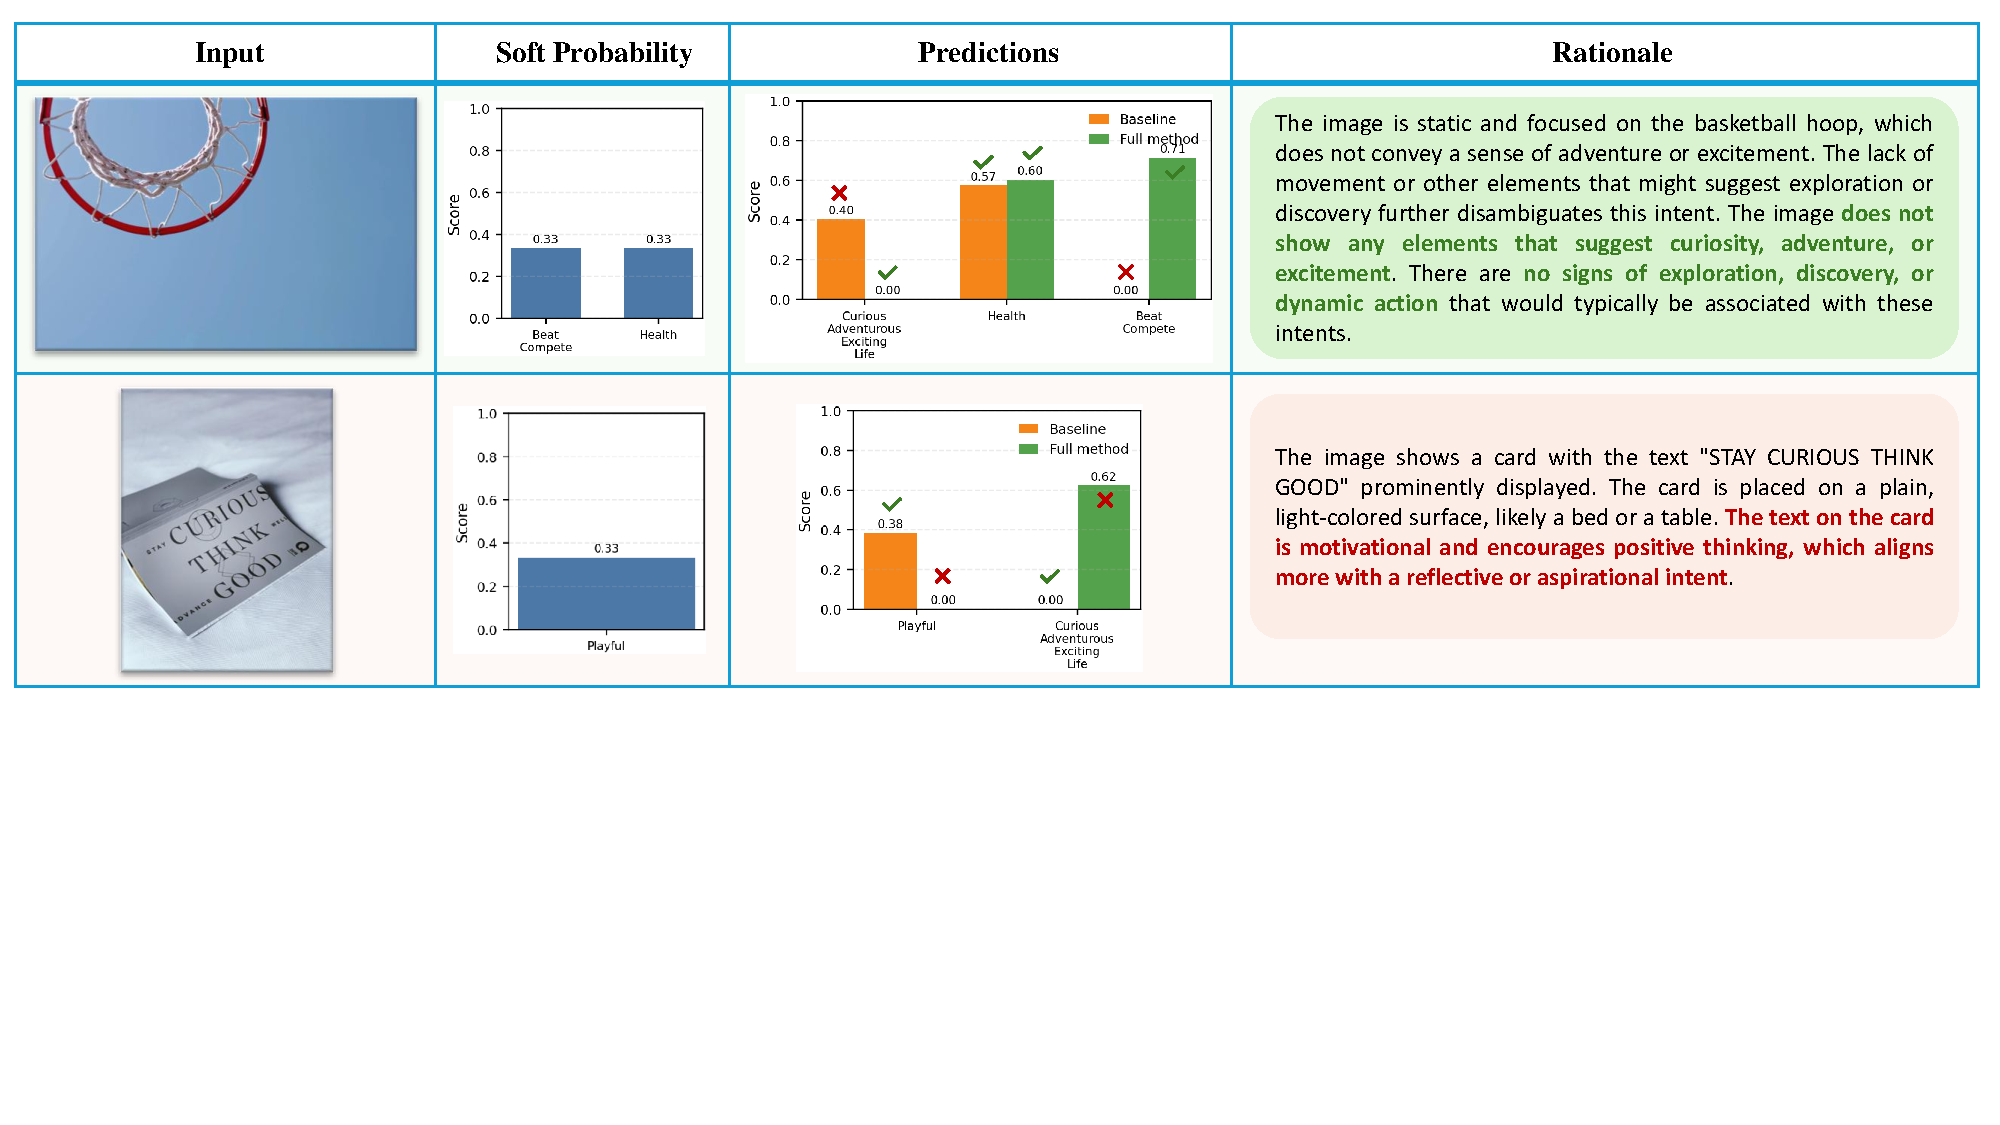
\includegraphics[width=\textwidth]{3_cases.pdf}
\caption{Qualitative case study of baseline and FDIL on representative Intentonomy samples.
% Top row: the baseline predicts an incorrect alternative, whereas FDIL rejects that distractor using counterfactual rationale evidence and recovers the correct intent. Bottom row: FDIL errs, but the soft label has only 0.33 agreement, so its alternative remains semantically plausible rather than arbitrary.
}
\label{fig:case_study}
\end{figure*}
